\addcontentsline{toc}{section}{Introduction}
\section{Introduction}
The objective of this section is to present the general context of the project, starting with the host organization, IZICAP, where I am completing my 5-month internship. We will describe their activities, strategy, values, as well as the organizational structure and profiles involved in my project. Then, we will address the work request that expresses the functional requirements on which I based the design and implementation of the solution, as well as the methodology followed to achieve the set objectives.

\section{Presentation of the Host Organization}
\subsection{IZICAP}
IZICAP is a unique and innovative company focused on data analysis, loyalty, and digital marketing for small and medium-sized enterprises (SMEs). Their user-friendly and easy-to-install solution is based on the SaaS model, allowing for the utilization of customers' transactional data from payment cards.

By collaborating with banks and acquirers, IZICAP offers an enhanced value proposition and provides a powerful digital marketing tool to SMEs. Their mission is to support merchants on a daily basis to accelerate the development of their businesses, thereby addressing their specific needs.

IZICAP's story dates back to 2013 when it emerged in an ever-evolving and increasingly complex landscape of financial services. Since then, traditional banking and payment models have been continually threatened by new, more innovative challenger companies. Intense competition means that merchant loyalty can no longer be taken for granted, and often acquirers and payment service providers are compelled to reduce their fees.

After establishing a strong presence in France through partnerships with Groupe BPCE and Crédit Agricole, Izicap formed a partnership with Nexi, the leading acquirer and fintech in Italy, and joined Mastercard's StartPath program with the aim of significantly expanding its global reach. This strategic expansion strengthens their position in the market and confirms their commitment to offering their services to a wider audience.

With Izicap, SMEs have access to an innovative solution that leverages data analysis to optimize their loyalty and marketing strategy. With their expertise and growing international presence, IZICAP is determined to support business growth and help them thrive in an ever-changing commercial environment.
\subsection{Strategic Partnerships}
IZICAP has established strategic partnerships with several key players in the financial industry. Among their notable partners are:
\begin{itemize}
\item \textbf{Groupe BPCE:} Izicap collaborated with Groupe BPCE, one of the leading banking groups in France, to provide their loyalty and digital marketing solution to merchants.
\item \textbf{Crédit Agricole:} Izicap partnered with Crédit Agricole, one of the largest French banks, to offer their services to merchants within their network.
\item \textbf{Nexi:} Izicap formed a partnership with Nexi, the leading acquirer and fintech company in Italy. This collaboration allows Izicap to expand its presence in the Italian market and benefit from Nexi's expertise in the field of payment services.
\item \textbf{Mastercard StartPath:} Izicap joined Mastercard's StartPath program, which supports startups and innovative companies in the fintech field. This collaboration provides Izicap with an opportunity to increase its visibility and expand internationally.
\item \textbf{BBVA:} Izicap also established a partnership with BBVA, one of the major banks in Spain and Latin America. This collaboration with BBVA strengthens Izicap's presence in the Spanish market and enables the company to offer its loyalty and digital marketing solutions to merchants affiliated with BBVA. The partnership with BBVA demonstrates Izicap's commitment to expanding its reach and working with major players in the financial industry to support small and medium-sized enterprises in their growth.
\item \textbf{Ingenico:} Izicap partnered with Ingenico, one of the leading providers of payment solutions and merchant services globally. Through this partnership, Izicap is able to integrate its loyalty and digital marketing solution into Ingenico's payment terminals, providing a comprehensive solution to merchants using Ingenico's services. This collaboration strengthens Izicap's position as a provider of innovative loyalty and marketing solutions, leveraging Ingenico's expertise and global reach in the payments industry.
\end{itemize}
\begin{figure}[H]
\centering
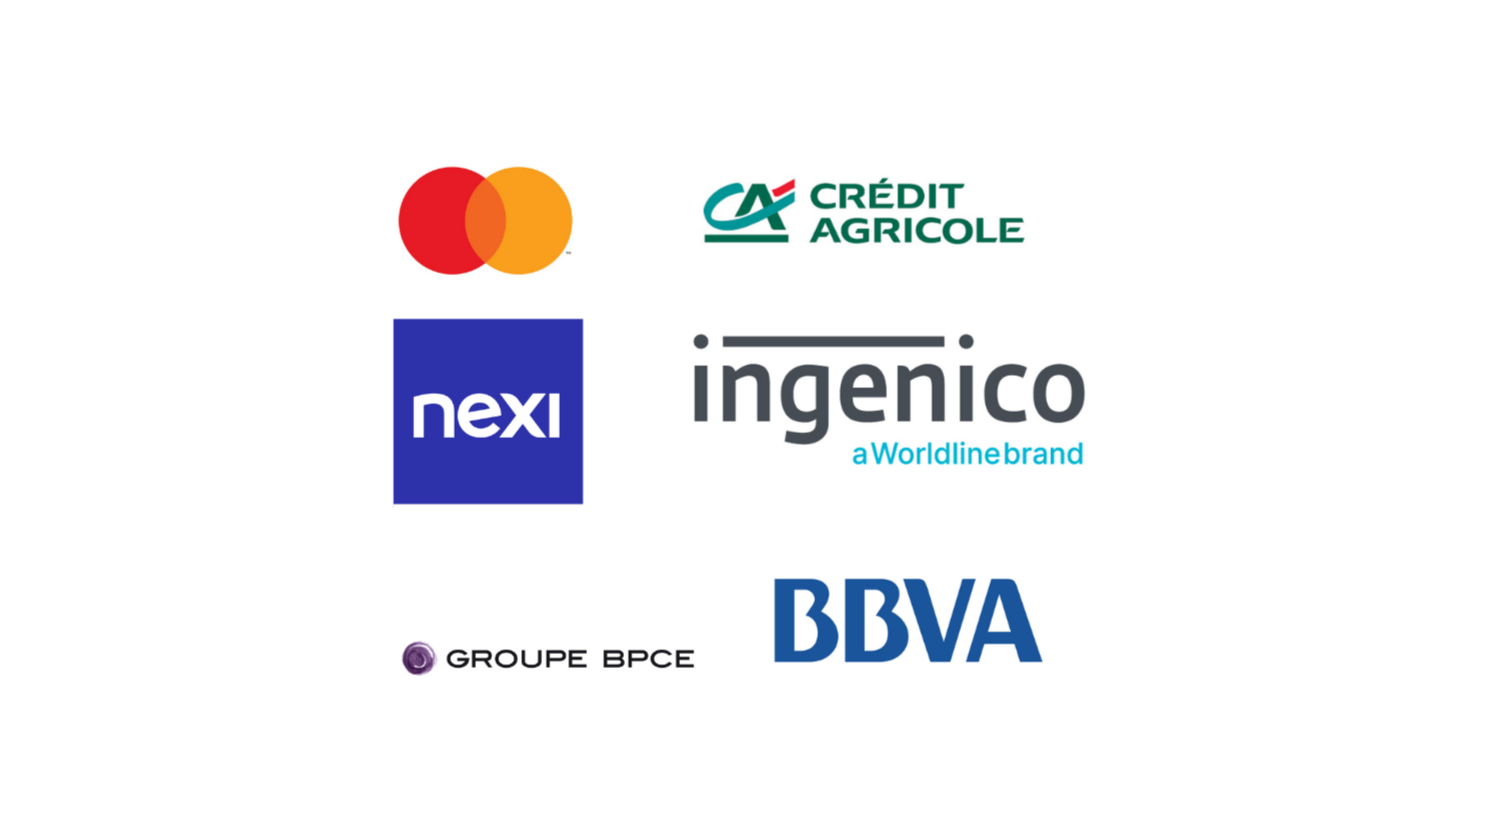
\includegraphics[width=\linewidth]{images/partenaires.png}
\caption{Strategic Partnerships}\label{fig:partnerships}
\end{figure}

\section{Organizational Structure}
\begin{figure}[H]
\centering
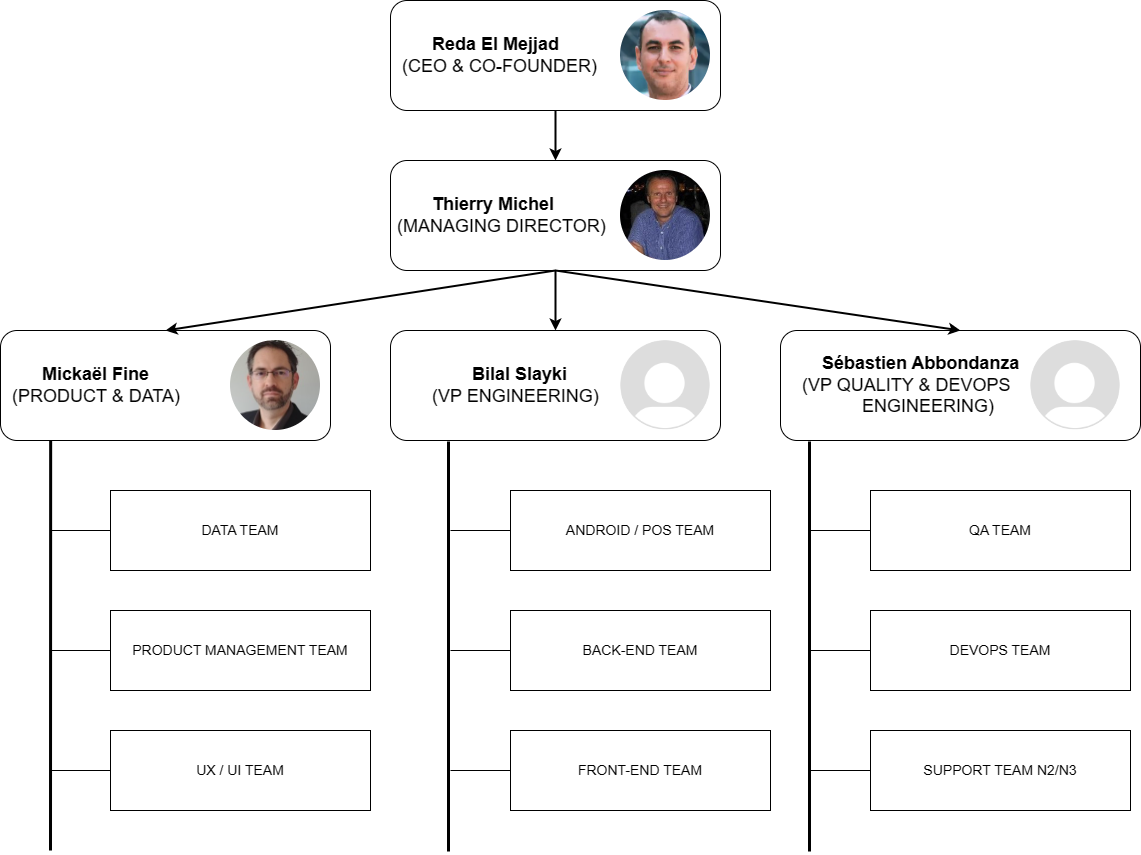
\includegraphics[width=0.75\linewidth]{images/organigram.png}
\caption{IZICAP Organizational Structure}\label{fig:organigram}
\end{figure}

Within the project team, I had the opportunity to work in a versatile manner across different domains. I actively contributed to backend development by participating in the design and implementation of microservices. I also collaborated with the frontend team, bringing my expertise in integrating microfrontends and improving the user experience. Additionally, I was involved in data management, contributing to the implementation of Delta Lake and optimizing data flows. This diverse experience allowed me to gain a holistic view of the project and effectively collaborate with different teams to achieve the set objectives.

\section{Project Framework}

The project involves the revamping of the "Smart data" application, which refers to the process of extracting valuable information from large amounts of data to make informed business decisions.

Smart data allows us to:

\begin{enumerate}
\item \textbf{Data collection}: Izicap helps businesses collect customer data from various touchpoints such as point-of-sale systems, loyalty programs, online interactions, etc. Ensure the integration of their data collection tools into your existing systems or processes.
\item \textbf{Data analysis}: Izicap's smart data solution enables you to analyze the collected data to discover trends, patterns, and customer behaviors. Use their analytics tools and algorithms to gain actionable insights from the data.
\item \textbf{Customer segmentation}: Segment your customer base based on their preferences, purchase history, demographic characteristics, or other relevant criteria. Izicap's smart data solution can assist you in identifying different customer segments and creating personalized marketing strategies for each segment.
\item \textbf{Personalized marketing}: Utilize the insights derived from Izicap's smart data solution to create targeted marketing campaigns. Send personalized offers, promotions, or recommendations to specific customer segments, thereby increasing the chances of conversion and customer satisfaction.
\item \textbf{Customer loyalty}: Leverage Izicap's smart data solution to identify customers who are at risk of churning or no longer making purchases from you. Develop loyalty strategies by offering incentives, loyalty programs, or personalized communications to keep them engaged and loyal to your brand.
\item \textbf{Performance tracking}: Regularly monitor the performance of your marketing campaigns and customer engagement efforts. Izicap's solution can provide you with metrics and reports to evaluate the effectiveness of your strategies and make data-driven adjustments when necessary.
\item \textbf{Continuous improvement}: Smart data solutions are most effective when used iteratively. Regularly analyze data, adapt your strategies, and refine your approach based on new insights and evolving customer behavior.
\end{enumerate}

\begin{figure}[H]
\centering
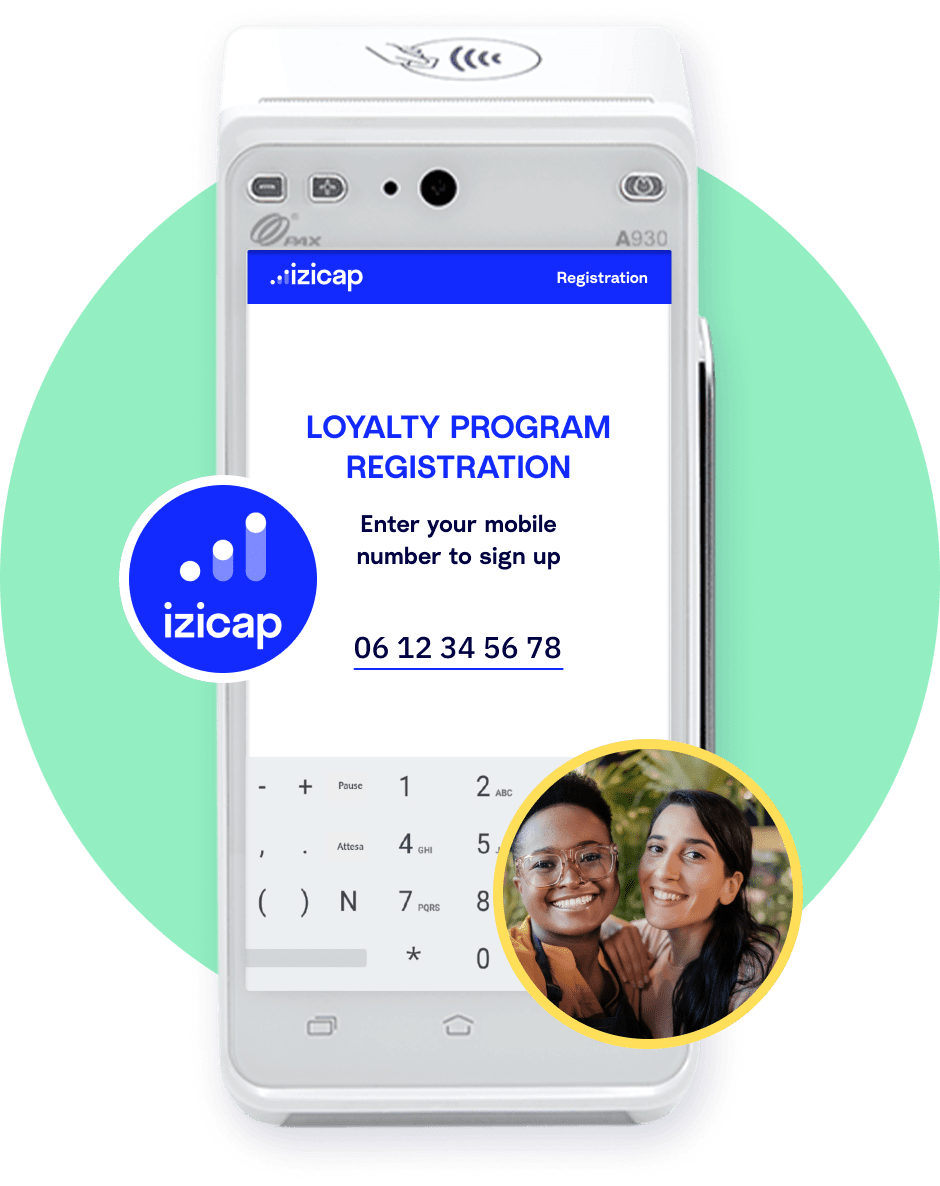
\includegraphics[width=0.6\linewidth]{images/smart-data-izicap.png}
\caption{Smart data Izicap}\label{fig:smart-data-Izicap}
\end{figure}

\section{System Architecture - Smart Data}

The figure below visualizes the structure and key components of our system, as well as the interactions between them. It forms the foundation of our system and plays a crucial role in providing features and services to our users.

\begin{figure}[H]
\centering
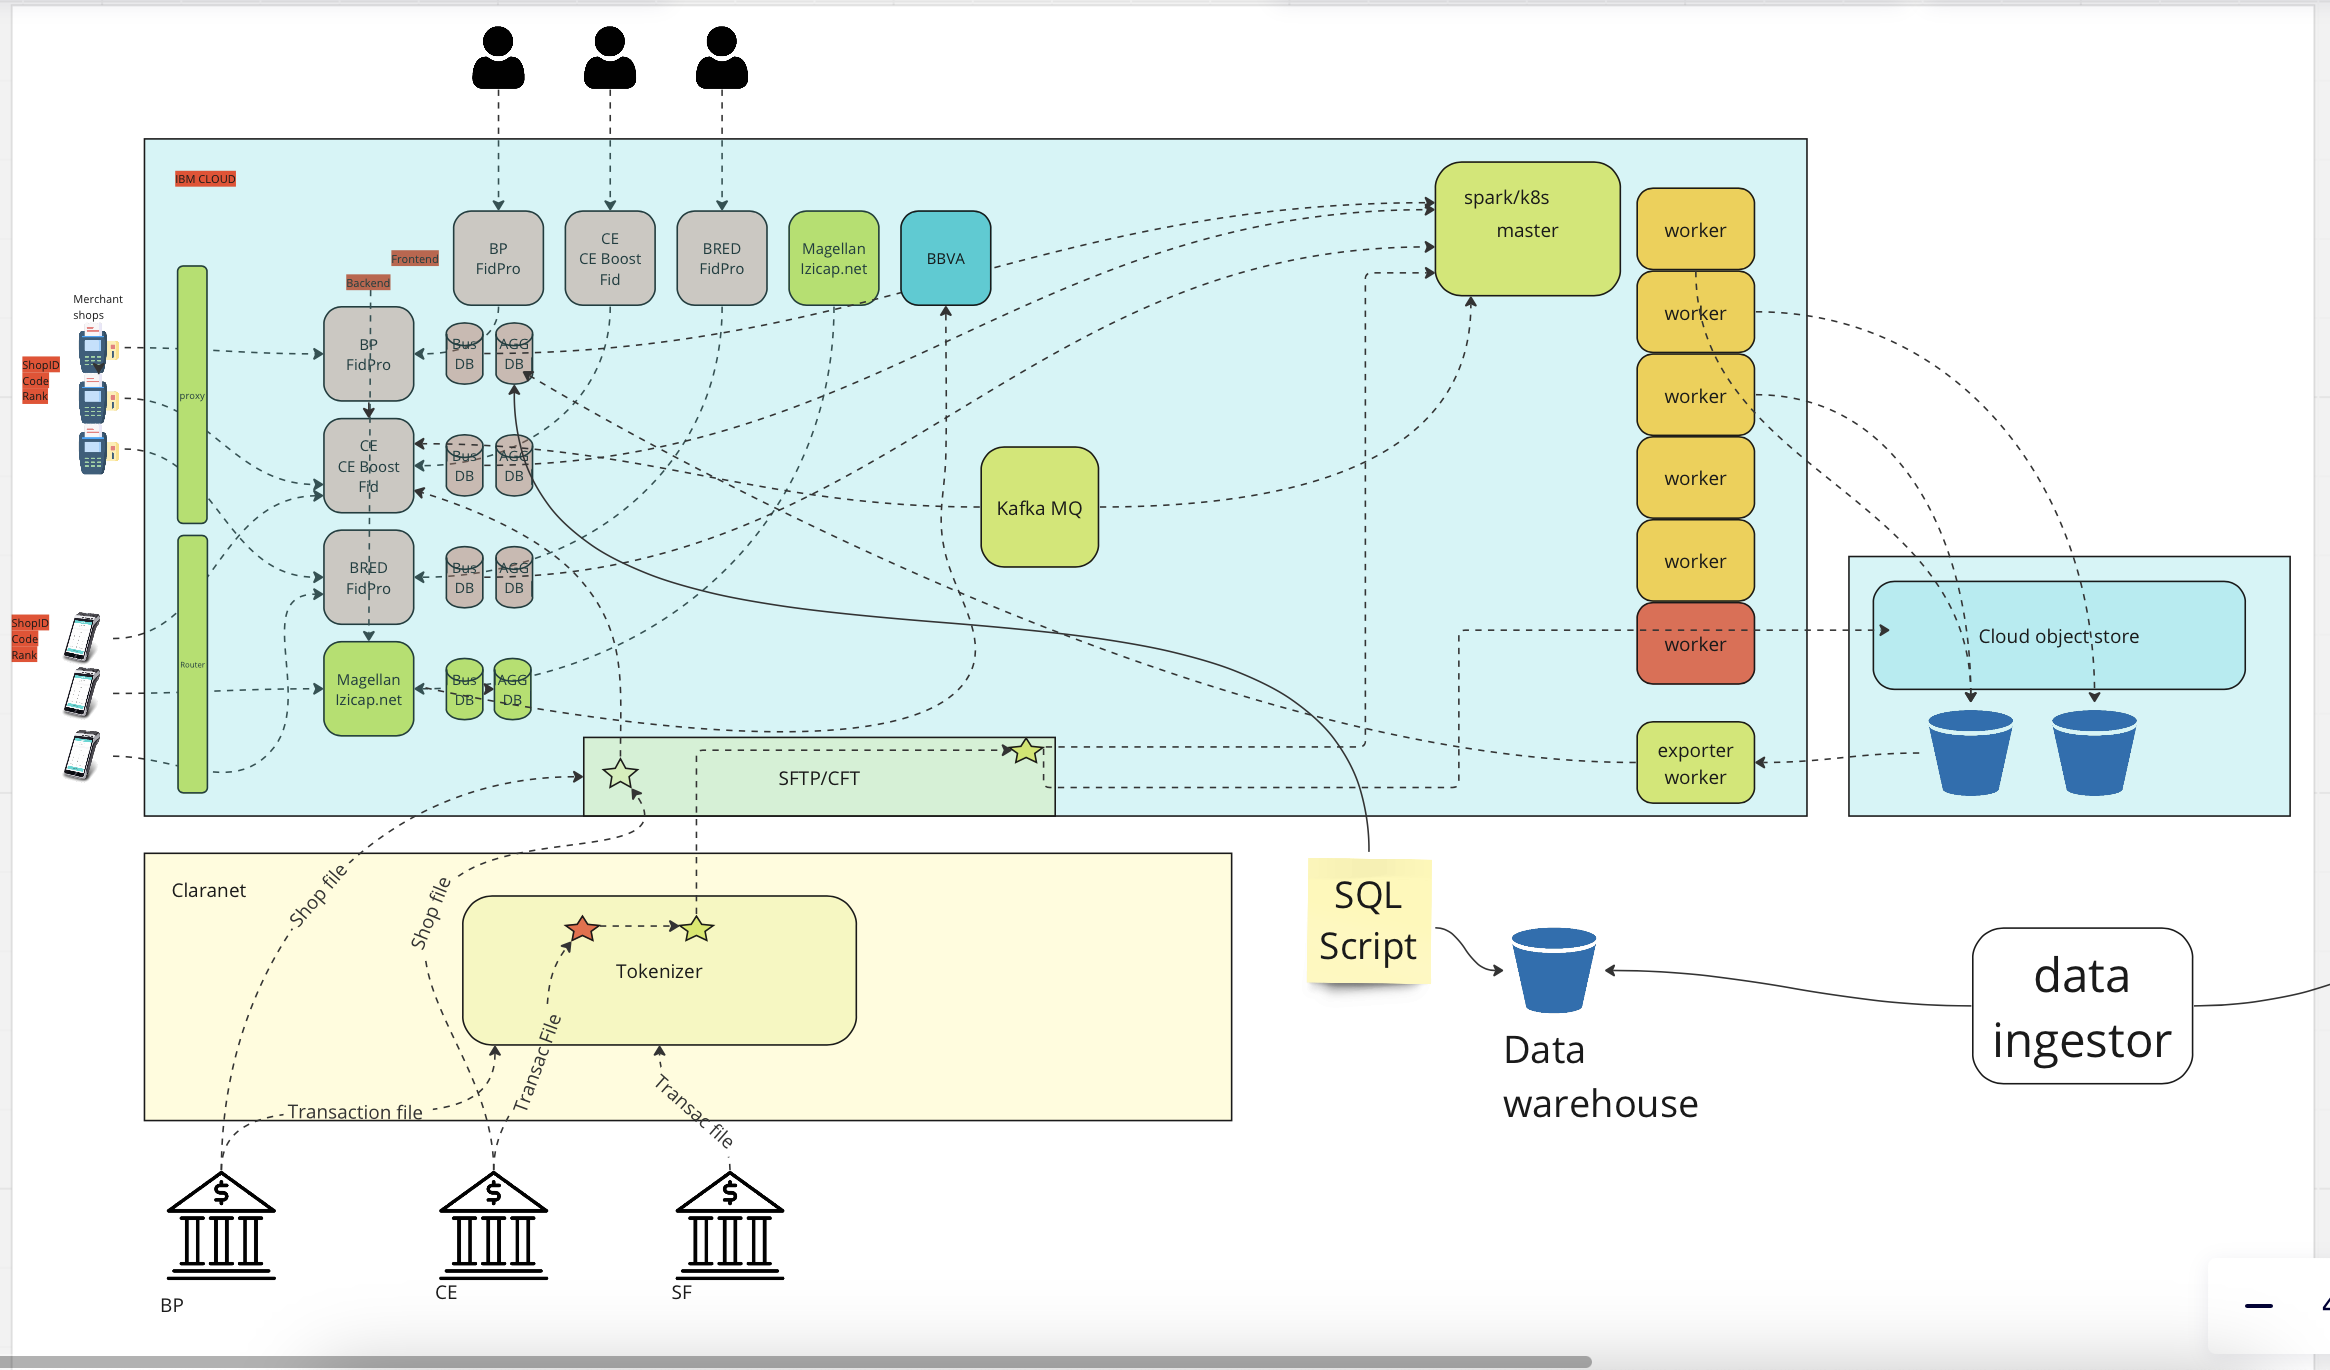
\includegraphics[width=\linewidth]{images/archi-globale.png}
\caption{Current System Architecture}\label{fig:monolithic-architecture}
\end{figure}

This diagram represents the functioning of the current monolithic architecture, which has several disadvantages that can hinder the efficiency, flexibility, and maintainability of the system. Here is a detailed description of the main drawbacks:

\begin{enumerate}
\item \textbf{Complexity and dependencies}: The monolithic architecture involves grouping all modules and functionalities of the system into a single block. This creates strong dependencies between different components, making understanding, management, and updates complex. Changes made to one part of the system can have repercussions on other parts, making testing, deployment, and bug fixing more challenging.
\item \textbf{Limited scalability}: Monolithic architecture often struggles to adapt to increased load or growing demand. Since all components are bundled into a single monolith, it is difficult to selectively scale a specific part of the system. This can lead to bottlenecks, reduced performance, and poor resource allocation when dealing with large data volumes or managing an increase in the number of users.
\item \textbf{Complex deployments and high risks}: With a monolithic architecture, deployments require updating the entire system, even for minor changes. This increases the risks of errors and regressions, as a single mistake can result in the unavailability of the entire system. Additionally, deployments need careful planning and coordination, which can lead to longer downtimes and service interruptions for users.
\item \textbf{Technological choice challenges}: In a monolithic architecture, the technologies used are often tightly coupled and integrated. This can make it difficult to adopt new technologies or integrate specialized components. Upgrading versions or adding new features can be limited by initial technological choices, hindering innovation and adaptation to market changes.
\item \textbf{Cohesion and responsibilities}: Monolithic architecture does not facilitate a clear separation of responsibilities and functionalities. Different modules of the system are often tightly coupled and may share common features. This makes isolating issues, module-specific maintenance, and code reuse specific to a domain challenging.
\end{enumerate}

\section{Problem and Functional Needs}

The problem at hand lies in the currently used monolithic architecture, which presents limitations in terms of scalability, flexibility, and maintainability. The constraints imposed by this architecture make it complex to deploy new functionalities and can potentially disrupt the entire system. Additionally, the use of a traditional relational database such as MariaDB proves insufficient for efficiently handling large volumes of transactional data. It is worth noting that the Smart Data application has been in existence for 10 years and has been developed using the Groovy language. This long period of existence attests to the stability and maturity of our system. However, the use of Groovy may present certain constraints in terms of maintainability and scalability, especially when it comes to integrating new technologies and managing more modern architectures.

\subsection*{Functional Needs}

To address these challenges, different functional needs have been identified:

\begin{enumerate}
\item[$\bullet$] \textbf{Scalability}: It is necessary to have an architecture that can easily adapt to a growing number of users, transactions, and data. It is essential that our system can scale harmoniously and maintain its performance even with a significant increase in workload.
\item[$\bullet$] \textbf{Flexibility}: We need to be able to introduce new functionalities independently and deploy them without disrupting the entire system. An approach based on microservices and microfrontends will enable us to achieve this flexibility by facilitating the development, testing, and isolated deployment of each component.
\item[$\bullet$] \textbf{Improved Performance}: It is crucial to have a data infrastructure capable of efficiently handling large volumes of transactional data. By replacing MariaDB with Delta Lake, we will be able to leverage advanced features such as ACID transaction management and compatibility with powerful analysis tools, significantly improving the performance and reliability of our system.
\item[$\bullet$] \textbf{Separation of Responsibilities}: We aim for better separation of responsibilities between different components of our system. Microservices will allow us to decouple functionalities, assign them to specific teams, and promote more effective code management, simplified maintenance, and increased scalability.
\end{enumerate}

\section{Internship Objectives}

The project falls within the scope of renewing the functionalities of the Smart Data application, aiming to improve its scalability, flexibility, and performance. In this context, the objectives of the internship are as follows:

\begin{enumerate}
\item Study and analyze the current architecture of the SMART DATA application to understand the constraints and limitations that hinder its growth and evolution.
\item Propose and design a migration strategy from the monolithic architecture to an architecture based on microservices and microfrontends, thus enabling better modularity and greater flexibility in the development and deployment of functionalities.
\item Implement multiple microservices with Spring Boot within the new architecture, using appropriate technology and ensuring its seamless integration with other components of the system.
\item Evaluate the benefits and implications of using Delta Lake as a replacement for the MariaDB database, with a focus on performance, transaction management, and integration with analysis tools.
\item Integrate Trino into the architecture to enable the execution of complex SQL queries and optimize data processing, ensuring effective collaboration with the development team.
\item Set up a deployment and management infrastructure for microservices, using tools such as Kubernetes, Docker, and Jenkins, to facilitate deployment, scaling, and component management.
\item Design and implement unit tests and integration tests to ensure the quality and reliability of the new components developed within the microservices-based architecture.
\item Thoroughly document the migration process and the technological choices made, providing clear instructions for the future maintenance of the architecture and management of updates.
\item Collaborate closely with the existing team to facilitate the transition to the new architecture, providing technical support, guidance, and training on the new technologies used.
\end{enumerate}

\section{Project Implementation Process}

The project implementation process followed several iterations called "sprints," typically lasting two weeks each. Each sprint focused on delivering functional increments of the application, enabling quick tangible results.

Here are the key steps of the project implementation process based on the Scrum methodology:

\begin{enumerate}
\item \textbf{Product backlog definition:} In collaboration with stakeholders and the development team, we identified and prioritized the features to be developed and integrated into the microservices-based architecture.
\item \textbf{Sprint planning:} At the beginning of each sprint, we held a planning meeting to define the specific sprint goals, select tasks to be accomplished, and estimate the required effort.
\item \textbf{Iterative development:} The development team worked iteratively on the assigned tasks, focusing on accomplishing the identified features for the current sprint.
\item \textbf{Daily stand-up meetings:} Every day, the team gathered for a brief stand-up meeting to share progress, potential obstacles, and coordinate activities.
\item \textbf{Sprint review:} At the end of each sprint, we conducted a sprint review to showcase the developed features and gather feedback from stakeholders. This allowed us to validate the achieved results and plan for the next steps.
\item \textbf{Sprint retrospective:} After the sprint review, we conducted a retrospective to evaluate the sprint's progress, identify strengths and areas for improvement, and adjust our approach accordingly.
\item \textbf{Subsequent iterations:} The planning, iterative development, sprint review, and retrospective process repeated for each subsequent sprint, enabling incremental progress towards the project's objectives.
\end{enumerate}

\begin{figure}[H]
\centering
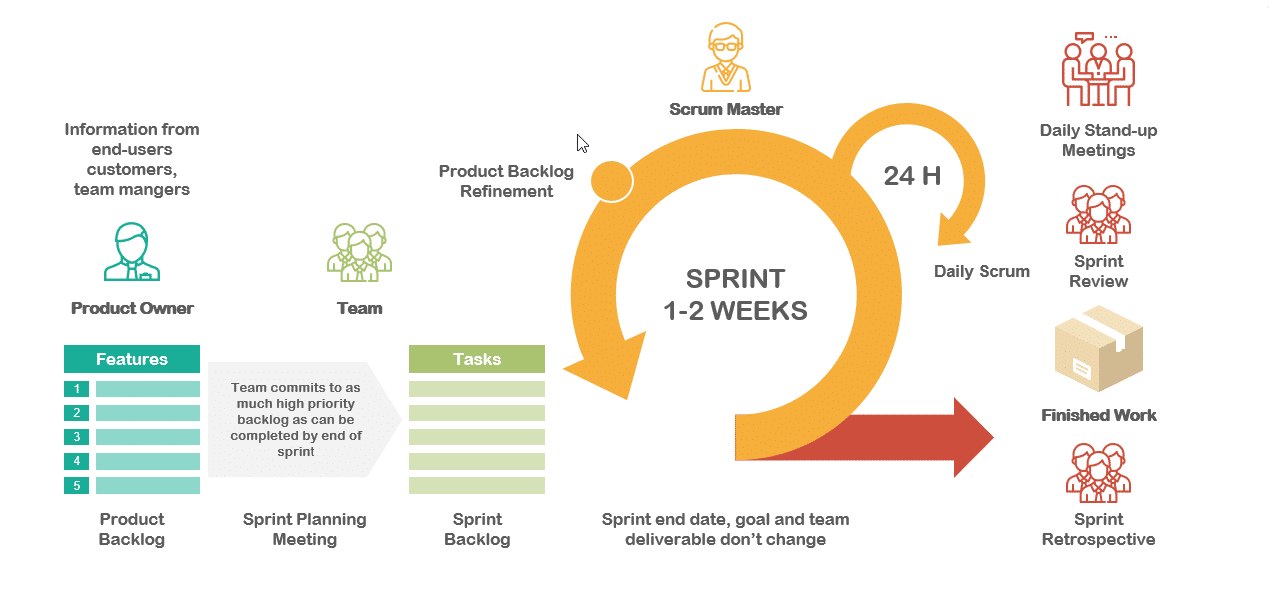
\includegraphics[width=\linewidth]{images/scrum.png}
\caption{Scrum Methodology}\label{fig:scrum}
\end{figure}

\section{Project Planning}
For the project planning, we used the method of modeling the network of task dependencies. This approach allowed us to break down the work into different structured tasks and establish dependency relationships between them.

We also utilized the technique of Gantt chart to graphically represent the project's tasks and resources over time. In the horizontal axis, we listed the different tasks, and in the vertical axis, we defined the days, weeks, or months. Each task was represented by a bar whose length was proportional to the estimated duration of that task.

The Gantt chart enabled us to visualize the distribution of tasks, their duration, and their sequence. Some tasks were performed sequentially, while others could be done in parallel, either partially or entirely. This clear and visual representation helped us plan the project by determining and organizing the different tasks to ensure effective project management.

The following figure presents the Gantt chart detailing the project's planning, with tasks arranged over time and their respective durations. This allowed us to track the project's progress, identify any delays, and take appropriate measures to resolve them.

\begin{figure}[H]
\centering
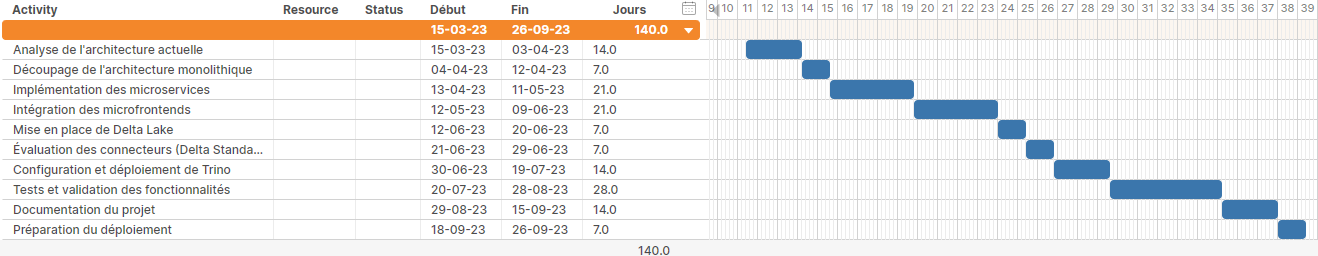
\includegraphics[width=\linewidth]{images/gantt.png}
\caption{Gantt Chart}\label{fig:gantt}
\end{figure}

\addcontentsline{toc}{section}{Conclusion}
\section*{Conclusion}

In conclusion of this section, we have presented the project planning for renewing the functionalities of the SMART DATA application. We developed a schedule based on the modeling of the network of task dependencies, using the technique of the Gantt chart. This chart allowed us to visualize the different activities, their estimated durations, and the required resources.

During the planning, we identified the main project activities, such as the analysis of the current architecture, decomposition of the monolithic architecture, implementation of microservices, integration of microfrontends, implementation of Delta Lake, evaluation of connectors, configuration and deployment of Trino, testing and validation of functionalities, project documentation, deployment preparation, as well as user training and awareness.

We also took into account the total duration of the project, which is estimated to be 5 months, and adjusted the durations of activities accordingly. This provided us with a more precise view of the project's temporal planning.